\documentclass[12pt]{article}
\usepackage{graphicx}
\usepackage{caption}
\usepackage{subcaption}
\usepackage{tikz}
\usepackage{tcolorbox}
\usepackage{listings}
\usepackage{amsmath}
\usepackage{amssymb}
\usepackage{xcolor}
\usepackage[margin=1cm, top=1.5cm, bottom=1.5cm]{geometry}

\tcbuselibrary{breakable}

\title{\textbf{Gráficas y Juegos: Tarea 01}}
\author{Martínez Méndez Ángel Antonio\\Pinzón Chan José Carlos\\Rendón Ávila Jesús Mateo}
\date{\today}

\begin{document}

\maketitle
\begin{center}
\vspace{3cm}
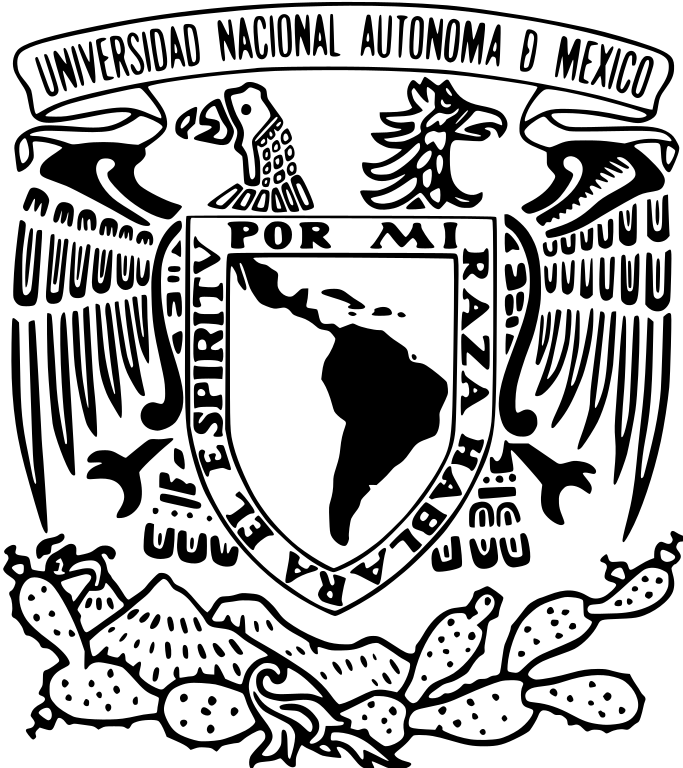
\includegraphics[width=0.195\textwidth]{Escudo.png}
\hspace{0.5cm}
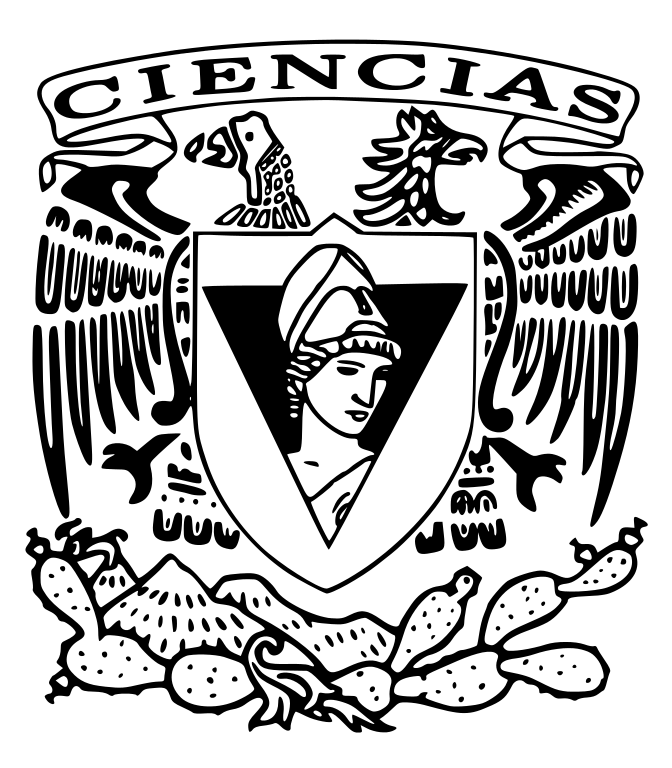
\includegraphics[width=0.2\textwidth]{logo_ciencias.png}
\end{center}
\begin{center}
    \vspace{1cm}
    Universidad Nacional Autónoma de México\\
    Facultad de Ciencias\\
    Profesor: César Hernández Cruz\\
\end{center}

\newpage

%
% Ejercicio 1
%
\textbf{1.} Dibuje todas las gráficas no isomorfas de cuatro vértices. Justifique brevemente por qué son
todas, es decir, justifique por qué la lista que exhibe es exhaustiva.

\vspace{1cm}

%Primera fila de graficas
\begin{figure}[h!]
    \centering
    \begin{minipage}{0.2\textwidth}
        \centering
        \begin{tikzpicture}[scale=1]
            \node (a) at (2,2) [circle,fill,inner sep=1.5pt] {};
            \node (b) at (0,2) [circle,fill,inner sep=1.5pt] {};
            \node (c) at (0,0) [circle,fill,inner sep=1.5pt] {};
            \node (d) at (2,0) [circle,fill,inner sep=1.5pt] {};
        \end{tikzpicture}
        \caption{Gráfica $G_1$}
    \end{minipage}
    \hspace{0.015\textwidth}
    \begin{minipage}{0.2\textwidth}
        \centering
        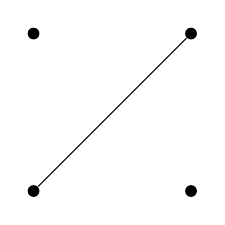
\begin{tikzpicture}[scale=1]
            \node (a) at (2,2) [circle,fill,inner sep=1.5pt] {};
            \node (b) at (0,2) [circle,fill,inner sep=1.5pt] {};
            \node (c) at (0,0) [circle,fill,inner sep=1.5pt] {};
            \node (d) at (2,0) [circle,fill,inner sep=1.5pt] {};
            \draw (a) -- (c);
        \end{tikzpicture}
        \caption{Gráfica $G_2$}
    \end{minipage}
    \hspace{0.015\textwidth}
    \begin{minipage}{0.2\textwidth}
        \centering
        \begin{tikzpicture}[scale=1]
            \node (a) at (2,2) [circle,fill,inner sep=1.5pt] {};
            \node (b) at (0,2) [circle,fill,inner sep=1.5pt] {};
            \node (c) at (0,0) [circle,fill,inner sep=1.5pt] {};
            \node (d) at (2,0) [circle,fill,inner sep=1.5pt] {};
            \draw (a) -- (b) (c) -- (d);
        \end{tikzpicture}
        \caption{Gráfica $G_3$}
    \end{minipage}
    \hspace{0.015\textwidth}
    \begin{minipage}{0.2\textwidth}
        \centering
        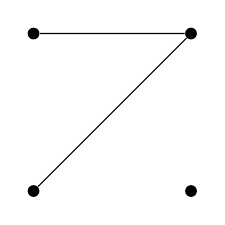
\begin{tikzpicture}[scale=1]
            \node (a) at (2,2) [circle,fill,inner sep=1.5pt] {};
            \node (b) at (0,2) [circle,fill,inner sep=1.5pt] {};
            \node (c) at (0,0) [circle,fill,inner sep=1.5pt] {};
            \node (d) at (2,0) [circle,fill,inner sep=1.5pt] {};
            \draw (a) -- (c) (a) -- (b);
        \end{tikzpicture}
        \caption{Gráfica $G_4$}
    \end{minipage}
\end{figure}

%segunda fila de graficas
\begin{figure}[h!]
    \centering
    \begin{minipage}{0.2\textwidth}
        \centering
        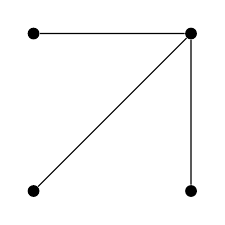
\begin{tikzpicture}[scale=1]
            \node (a) at (2,2) [circle,fill,inner sep=1.5pt] {};
            \node (b) at (0,2) [circle,fill,inner sep=1.5pt] {};
            \node (c) at (0,0) [circle,fill,inner sep=1.5pt] {};
            \node (d) at (2,0) [circle,fill,inner sep=1.5pt] {};
            \draw (a) -- (b) (a) -- (c) (a) -- (d);
        \end{tikzpicture}
        \caption{Gráfica $G_5$}
    \end{minipage}
    \hspace{0.015\textwidth}
    \begin{minipage}{0.2\textwidth}
        \centering
        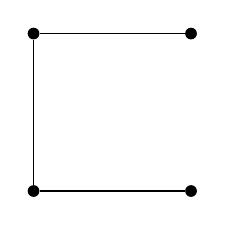
\begin{tikzpicture}[scale=1]
            \node (a) at (2,2) [circle,fill,inner sep=1.5pt] {};
            \node (b) at (0,2) [circle,fill,inner sep=1.5pt] {};
            \node (c) at (0,0) [circle,fill,inner sep=1.5pt] {};
            \node (d) at (2,0) [circle,fill,inner sep=1.5pt] {};
            \draw (a) -- (b) (b) -- (c) (c) -- (d);
        \end{tikzpicture}
        \caption{Gráfica $G_6$}
    \end{minipage}
    \hspace{0.015\textwidth}
    \begin{minipage}{0.2\textwidth}
        \centering
        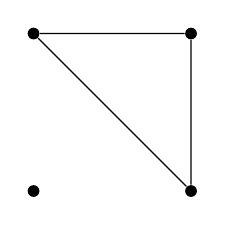
\begin{tikzpicture}[scale=1]
            \node (a) at (2,2) [circle,fill,inner sep=1.5pt] {};
            \node (b) at (0,2) [circle,fill,inner sep=1.5pt] {};
            \node (c) at (0,0) [circle,fill,inner sep=1.5pt] {};
            \node (d) at (2,0) [circle,fill,inner sep=1.5pt] {};
            \draw (a) -- (b) (b) -- (d) (a) -- (d);
        \end{tikzpicture}
        \caption{Gráfica $G_7$}
    \end{minipage}
    \hspace{0.015\textwidth}
    \begin{minipage}{0.2\textwidth}
        \centering
        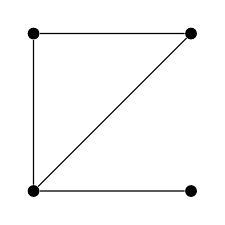
\begin{tikzpicture}[scale=1]
            \node (a) at (2,2) [circle,fill,inner sep=1.5pt] {};
            \node (b) at (0,2) [circle,fill,inner sep=1.5pt] {};
            \node (c) at (0,0) [circle,fill,inner sep=1.5pt] {};
            \node (d) at (2,0) [circle,fill,inner sep=1.5pt] {};
            \draw (a) -- (c) (a) -- (b) (b) -- (c) (c) -- (d);
        \end{tikzpicture}
        \caption{Gráfica $G_8$}
    \end{minipage}
\end{figure}

%tercera fila de graficas
\begin{figure}[h!]
    \centering
    \begin{minipage}{0.2\textwidth}
        \centering
        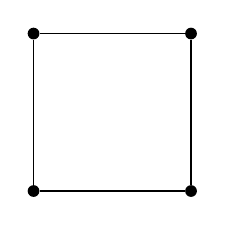
\begin{tikzpicture}[scale=1]
            \node (a) at (2,2) [circle,fill,inner sep=1.5pt] {};
            \node (b) at (0,2) [circle,fill,inner sep=1.5pt] {};
            \node (c) at (0,0) [circle,fill,inner sep=1.5pt] {};
            \node (d) at (2,0) [circle,fill,inner sep=1.5pt] {};
            \draw (a) -- (b) (a) -- (d) (b) -- (c) (c) -- (d);
        \end{tikzpicture}
        \caption{Gráfica $G_9$}
    \end{minipage}
    \hspace{0.015\textwidth}
    \begin{minipage}{0.2\textwidth}
        \centering
        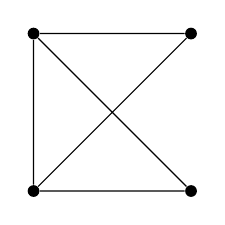
\begin{tikzpicture}[scale=1]
            \node (a) at (2,2) [circle,fill,inner sep=1.5pt] {};
            \node (b) at (0,2) [circle,fill,inner sep=1.5pt] {};
            \node (c) at (0,0) [circle,fill,inner sep=1.5pt] {};
            \node (d) at (2,0) [circle,fill,inner sep=1.5pt] {};
            \draw (a) -- (b) (a) -- (c) (b) -- (c) (b) -- (d) (c) -- (d);
        \end{tikzpicture}
        \caption{Gráfica $G_10$}
    \end{minipage}
    \hspace{0.015\textwidth}
    \begin{minipage}{0.2\textwidth}
        \centering
        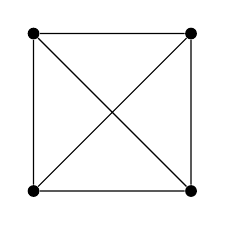
\begin{tikzpicture}[scale=1]
            \node (a) at (2,2) [circle,fill,inner sep=1.5pt] {};
            \node (b) at (0,2) [circle,fill,inner sep=1.5pt] {};
            \node (c) at (0,0) [circle,fill,inner sep=1.5pt] {};
            \node (d) at (2,0) [circle,fill,inner sep=1.5pt] {};
            \draw (a) -- (b) (a) -- (c) (b) -- (c) (c) -- (d) (b) -- (d) (a) -- (d);
        \end{tikzpicture}
        \caption{Gráfica $G_11$}
    \end{minipage}
\end{figure}

Parece haber un patrón en la forma de dibujar las gŕaficas:\\

Para 0 y 6 aristas se tiene una sola posibilidad de gráfica. Lo mismo sucede para las graficas de 1 y 5 aristas.\\

Ahora, para las gráficas de 2 y 4 aristas se tienen dos posibilidades de gráfica para cada una. Ya sea añadiendo una arista a la grafica de secuencia
de grados $[1, 1, 0, 0]$, vemos que podemos añadir la nueva arista tal que
tenga un extremo en un vértice con $d(V(G)) = 1$ o $d(V(G)) = 0$, 
de forma que no repitan las aristas existentes, de ahí las 2 posibilidades de graficas.\\

Este proceso aplica para la gráfica de 5 aristas, cuya secuencia de grados es $[3, 3, 2, 2,]$, vemos
que podemos aliminar una arista tal que tenga un extremo en un vértice con $d(V_g) = 2$ o $d(V_g) = 3$\\

De las gráficas anteriormente obtenidas, ya sea quitando o añadiendo aristas, 
ahora tendremos secuencias de grados con tres posibilidades para colocar nuevas aristas,
de ahí que para 3 aristas tenemos 3 posibles gráficas.\\
\vspace{1cm}

%
% Ejercicio 2
%
\textbf{2.} Sean $G$ y $H$ gráficas.
\\
\\
\textbf{a)} Demuestre que $G$ es isomorfa a $H$ si y sólo si $\overline{G}$ es isomorfa a $\overline{H}$.\\
$\Rightarrow)$
\begin{tcolorbox}[title=\textbf{Hipotesis}, colback=red!15!white, colframe=black!, breakable]
    $G$ es isomorfa a $H$.
\end{tcolorbox}
\begin{tcolorbox}[title=\textbf{Definiciones}, colback=blue!15!white, colframe=black!, breakable]
    $Def$. Una gráfica $G$ es \textbf{isomorfa} a una gráfica $H$ si existe una función $\varphi$ biyectiva, tal que:
    \[\varphi: V(G) \rightarrow V(H)\]
    Tal que para cualesquiera vertices $u,v \in V(G)$, se cumple que:
    \[uv \in E(G) \Leftrightarrow \varphi(u)\varphi(v) \in E(H)\]
    \\
    $Def$.El \textbf{complemento} de una gráfica $G$, denotada como $\overline{G}$, es la gráfica con el conjunto de vértices:
    \[V(\overline{G}) = V(G)\]
    y el conjunto de aristas:
    \[E(\overline{G}) = \{ uv \in V(G) \times V(G) \mid uv \notin E(G)\}\]
\end{tcolorbox}

$P.D$.
\[\overline{G} \cong \overline{H}\]
Tenemos que encontrar una función $?$ que satisfaga la definición de isomorfismo para $\overline{G}$ y $\overline{H}$.\\
Como por nuestra Hipotesis sabemos que $G \cong H$ entonces existe una funcion $\varphi$ biyectiva.\\
\\
Por definición de complemento de una gráfica, tenemos que:
\[V(\overline{G}) = V(G) \text{ y } V(\overline{H}) = V(H)\] 
y
\[E(\overline{G}) = \{ uv \in V(G) \times V(G) \mid uv \notin E(G)\} \text{ y } E(\overline{H}) = \{ uv \in V(H) \times V(H) \mid uv \notin E(H)\}\]
\\
Con ello podemos proponer la misma función $\varphi$ para el isomorfismo de $\overline{G}$ y $\overline{H}$, ya que por definición de complemento $V(G) = V(\overline{G})$ y $V(H) = V(\overline{H})$,
tenemos aśi que:
\[\varphi: V(\overline{G}) \rightarrow V(\overline{H})\]
que cumple, de nuevo por definición de complemento:
\[\text{Si } uv \notin E(G) \Longleftrightarrow \varphi(u)\varphi(v) \notin E(H) \]
\[\text{entonces, por def. de complemento } uv \in E(\overline{G}) \Longleftrightarrow \varphi(u)\varphi(v) \in E(\overline{H})\]
\\
Por lo tanto, $\overline{G} \cong \overline{H}$. 
\\
\\
$\Leftarrow)$\\
La demostración es analoga a la anterior, simplemente intercambiando $V(G)$ por $V(\overline{G})$ y $V(H)$ por $V(\overline{H})$.
\\
\\
\textbf{b)} Usando la definición de conexidad vista en clase, demuestre que si $G$ es inconexa,
entonces $\overline{G}$ es conexa.
\begin{tcolorbox}[title=\textbf{Hipotesis}, colback=red!15!white, colframe=black!]
    $G$ es inconexa, lo que implica la negación de conexidad.
\end{tcolorbox}
\begin{tcolorbox}[title=\textbf{Definiciones}, colback=blue!15!white, colframe=black!]
    $Def$. Una grafica $G$ es \textbf{conexa} si para cualquier partición $(X,Y)$ de $V(G)$, existe al menos una arista con un extremo
    en $X$ y el otro en $Y$.
\end{tcolorbox}
$P.D.$ \[\overline{G} \text{ es conexa.}\]
Sea una gráfica $G$ inconexa, bajo cualquier partición $(X,Y)$ de $V(G)$, no existe una arista
con un extremo en $X$ y el otro en $Y$.\\
\\
De lo anterior, aseguramos que el complemento de $G$, denotado por $\overline{G}$, debe ser conexa, ya que bajo la partición $(X,Y)$ de $V(G)$
existe al menos una arista con un extremo en $X$ y el otro en $Y$.\\
\\
Por lo tanto, $\overline{G}$ es conexa.
\vspace{1cm}

%
% Ejercicio 3
%
\textbf{3.} Sea $D$ una digráfica. Utilizando un análogo para digráficas de las matrices de incidencia, dmeuestra que:\\
\[
\sum_{\displaystyle v \in V_D} d^{+}(v) = \sum_{\displaystyle v \in V_D} d^{-}(v) = |A_D|
\]
\begin{tcolorbox}[title=\textbf{Hipotesis}, colback=red!15!white, colframe=black!]
    $D$ es una gŕafica dirigida (digráfica).
\end{tcolorbox}
\begin{tcolorbox}[title=\textbf{Definiciones}, colback=blue!15!white, colframe=black!]
    $Def$. Una gráfica $D$ es una \textbf{gráfica dirigida} si $D$ es una pareja ordenada $D=(V,A)$, donde
    $V$ es un conjunto arbitrario y $A$ es un subconjunto de $V \times V$ (parejas ordenadas).
    \\
    \\
    $Def$. La \textbf{matríz de incidencia} $M$ de $G$ es la matriz de $m \times n$ con entradas en $\{0, 1\}$ tal que:
    \[M_{ij} = \begin{cases} 1 & \text{si el vértice } v_i \in e_j\\ 0 & \text{en otro caso} \end{cases}\]

\end{tcolorbox}

$P.D.$
\[\sum_{\displaystyle v \in V_D} d^{+}(v) = \sum_{\displaystyle v \in V_D} d^{-}(v) = |A_D|\]
Sea $M^+$ y $M^-$ las matrices de incidencia de los exgrados e ingrados respectivamente, si tenemos una gráfica dirigida $D$ y su conjunto
de vértices $V(D)$ tal que:
\[V(D) = \{v_1, v_2, ..., v_n\}\]
y su conjunto de aristas $A(D)$ tal que:
\[A(D) = \{e_1, e_2, ..., e_m\}\]
Para la matríz de incidencia de una digráfica, tanto para los exgrados e ingrados, la suma
de los elementos de cada columna es igual a $1$. Sea la suma de los elementos de la columna igual a $0$,
se concluye que la arista no existe, por otro lado, si la suma es igual a $1$, la arista \textit{sale} de algún vértice (exgrado)
o se dirige a algún vértice (ingrado).\\

Suponiendo que la suma de la columna sea $\geq 2$, esto no es posible puesto que una arista sólo puede partir de un solo punto y viceversa, $i.e$ sólo 
puede dirigirse a un solo punto.\\

Como resultado al sumar todas las columnas de $M^+$ o $M^-$ obtenemos el número de aristas de la gráfica, $i.e$ se obtiene la 
cardinalidad de $A(D)$.

De forma similar, si sumamos las entradas del $i-esimo$ renglón de $M^+$ obtenemos el exgrado (o ingrado en el caso de $M^-$) del vértice $v_i$.\\

En base a lo anterior se puede argumentar que:
\[\mid A(D) \mid = \sum\limits_{j = 1}^{m} 1\]
\[= \sum\limits_{j = 1}^{m} \sum\limits_{n = 1}^{n} M^+_{ij}\]
\[= \sum\limits_{i = 1}^{n} \sum\limits_{j = 1}^{m} M^+_{ij}\]
\[= \sum\limits_{i = 1}^{n} d^+(v_i)\]
\[= \sum\limits_{i = 1}^{n} d^+(v_i)\]
\[= \sum_{\displaystyle v \in V(D)} d^+(v_i)\] 
Analogamente podemos hacerlo para ingrados, por lo que:
\[\mid A(D) \mid = \sum_{\displaystyle v \in V(D)} d^+(v) = \sum_{\displaystyle v \in V(D)} d^-(v)\]



\vspace{1cm}
%
% Ejercicio 4
%
\textbf{4.} Sea $n$ un entero positivo. Definimos la \textit{Retícula Boleana, BL\_n}, como
la gráfica cuyo conjunto de vértices es el conjunto de todos los posibles subconjuntos
de $\{1, ..., n\}$, donde dos subconjuntos $X$ y $Y$ son adyacentes si y sólo si su diferencia
tiene exactamente un elemento.\\
\\
\textbf{(a)} Dibuje $BL_1$, $BL_2$, $BL_3$ y $BL_4$.
\\

Para $BL_1$ tenemos que el conjunto de vértices $V$ es el conjunto de todos los posibles subconjuntos de $\{1\}$, es decir:
\[V(BL_1) = \{\emptyset, \{1\}\}\]

\begin{figure}[h!]
    \centering
    \begin{minipage}{0.4\textwidth}
        \centering
        
\begin{tikzpicture}[scale=1]
            \node (a) at (0,0) [circle,fill,inner sep=1.5pt] {};
            \node (b) at (0,1) [circle,fill,inner sep=1.5pt] {};

            \draw (a) -- (b);
        \end{tikzpicture}
        \caption{Gráfica de $BL_1$}
    \end{minipage}
\end{figure}

Para $BL_2$ tenemos que el conjunto de vértices $V$ es el conjunto de todos los posibles subconjuntos de $\{1, 2\}$, es decir:
\[V(BL_2) = \{\emptyset, \{1\}, \{2\} \{1, 2\}\}\]

\begin{figure}[h!]
    \centering
    \begin{minipage}{0.4\textwidth}
        \centering
        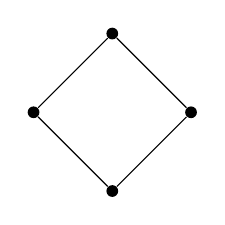
\begin{tikzpicture}[scale=1]
            \node (a) at (1,0) [circle,fill,inner sep=1.5pt] {};
            \node (b) at (0,1) [circle,fill,inner sep=1.5pt] {};
            \node (c) at (2,1) [circle,fill,inner sep=1.5pt] {};
            \node (d) at (1,2) [circle,fill,inner sep=1.5pt] {};

            \draw (a) -- (b) (a) -- (c) (b) -- (d) (c) -- (d);
        \end{tikzpicture}
        \caption{Gráfica de $BL_2$}
    \end{minipage}
\end{figure}

Para $BL_3$ tenemos que el conjunto de vértices $V$ es el conjunto de todos los posibles subconjuntos de $\{1, 2, 3\}$, es decir:
\[V(BL_3) = \{\emptyset, \{1\}, \{2\}, \{3\}, \{1, 2\}, \{1, 3\}, \{2, 3\},\{1, 2, 3\}\}\]

\begin{figure}[h!]
    \centering
    \begin{minipage}{0.4\textwidth}
        \centering
        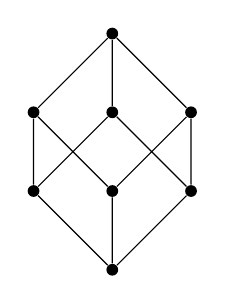
\begin{tikzpicture}[scale=1]
            \node (a) at (1,0) [circle,fill,inner sep=1.5pt] {};
            \node (b) at (0,1) [circle,fill,inner sep=1.5pt] {};
            \node (c) at (1,1) [circle,fill,inner sep=1.5pt] {};
            \node (d) at (2,1) [circle,fill,inner sep=1.5pt] {};
            \node (e) at (0,2) [circle,fill,inner sep=1.5pt] {};
            \node (f) at (1,2) [circle,fill,inner sep=1.5pt] {};
            \node (g) at (2,2) [circle,fill,inner sep=1.5pt] {};
            \node (h) at (1,3) [circle,fill,inner sep=1.5pt] {};

            \draw (a) -- (b) (a) -- (c) (a) -- (d) (b) -- (e) (b) --(f) (c) -- (e) (c) -- (g) (d) -- (f) (d) -- (g) (e) -- (h) (f) -- (h) (g) -- (h);
        \end{tikzpicture}
        \caption{Gráfica de $BL_3$}
    \end{minipage}
\end{figure}

Para $BL_4$ tenemos que el conjunto de vértices $V$ es el conjunto de todos los posibles subconjuntos de $\{1, 2, 3, 4\}$, es decir:
\[V(BL_4) = \{\emptyset, \{1\}, \{2\}, \{3\}, \{4\}, \{1, 2\}, \{1, 3\}, \{1, 4\}, \{2, 3\}, \{2, 4\},\]
\[\{3, 4\}, \\\{1, 2, 3\}, \{1, 3, 4\}, \{1, 2, 4\}, \{2, 3, 4\}, \{1, 2, 3, 4\}\}\]
\newpage
\begin{figure}[h!]
    \centering
    \begin{minipage}{0.4\textwidth}
        \centering
        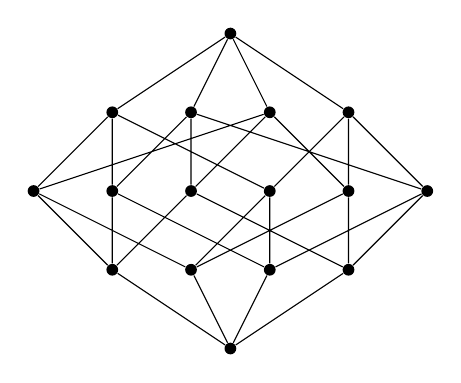
\begin{tikzpicture}[scale=1]
            \node (a) at (2.5,0) [circle,fill,inner sep=1.5pt] {};
            \node (b) at (1,1) [circle,fill,inner sep=1.5pt] {};
            \node (c) at (2,1) [circle,fill,inner sep=1.5pt] {};
            \node (d) at (3,1) [circle,fill,inner sep=1.5pt] {};
            \node (e) at (4,1) [circle,fill,inner sep=1.5pt] {};
            \node (f) at (0,2) [circle,fill,inner sep=1.5pt] {};
            \node (g) at (1,2) [circle,fill,inner sep=1.5pt] {};
            \node (h) at (2,2) [circle,fill,inner sep=1.5pt] {};
            \node (i) at (3,2) [circle,fill,inner sep=1.5pt] {};
            \node (j) at (4,2) [circle,fill,inner sep=1.5pt] {};
            \node (k) at (5,2) [circle,fill,inner sep=1.5pt] {};
            \node (l) at (1,3) [circle,fill,inner sep=1.5pt] {};
            \node (m) at (2,3) [circle,fill,inner sep=1.5pt] {};
            \node (n) at (3,3) [circle,fill,inner sep=1.5pt] {};
            \node (o) at (4,3) [circle,fill,inner sep=1.5pt] {};
            \node (p) at (2.5,4) [circle,fill,inner sep=1.5pt] {};

            \draw (a) -- (b) (a) -- (c) (a) -- (d) (a) -- (e) (b) -- (f) (b) -- (g) (b) -- (h) (c) -- (f) (c) -- (i) (c) -- (j) (d) -- (g) (d) -- (i) (d) -- (k) (e) -- (h) (e) -- (j) (e) -- (k) (f) -- (l) (f) -- (n) (g) --(l) (g) -- (m) (h) -- (m) (h) -- (n) (i) -- (l) (i) -- (o) (j) -- (n) (j) -- (o) (k) -- (m) (k) -- (o) (l) -- (p) (m) -- (p) (n) -- (p) (o) -- (p);
        \end{tikzpicture}
        \caption{Gráfica de $BL_4$}
    \end{minipage}
\end{figure}

\textbf{b)} Determine $|V_{BL_n}|$ y $|E_{BL_n}|$ (Demuestre su respuesta).

\begin{tcolorbox}[title=\textbf{Definiciones}, colback=blue!15!white, colframe=black!]
    $Def$. Sea $A$ un conjunto, definimos al \textbf{conjunto potencia} de $A$, denotado como $\mathcal{P}(A)$, como el conjunto de todos los subconjuntos de $A$. $i.e$:
    \[\mathcal{P}(A) = \{X \mid X \subseteq A\}\]
\end{tcolorbox}
Como sabemos que $V_{BL_n}$ es el conjunto de todos los posibles subconjuntos de $\{1, ..., n\}$, entonces
podemos verlo como el conjunto potencia de $\{1, ..., n\}$, es decir:
\[V_{BL_n} = \mathcal{P}(\{1, ..., n\})\]
cuya cardinalidad se define como:
\[|V_{BL_n}| = 2^n\]

El primer producto $n$ representa las aristas que hay en los vertices de los extremos de la gráfica,
en este caso $\varnothing$ y $\{1, 2, ... , n\}$

\textbf{c)} Demuestre que $BL_n$ es bipartita para cualquier $n \in \mathbb{Z} \text{ tal que } n > 0$.

\begin{tcolorbox}[title=\textbf{Definiciones}, colback=blue!15!white, colframe=black!]
    $Def$. Sea $n$ un entero positivo. la \textbf{Retícula Boleana, BL\_n}, como
    la gráfica cuyo conjunto de vértices es el conjunto de todos los posibles subconjuntos
    de $\{1, ..., n\}$, donde dos subconjuntos $X$ y $Y$ son adyacentes si y sólo si su diferencia
    tiene exactamente un elemento.\\

    $Def.$ Una gráfica $G$ es \textbf{bipartita} si $V(G)$ admite una patición $V = (X, Y)$ tal que $X$ y $Y$ son conjuntos independientes.
\end{tcolorbox}

$P.D$ $BL_N$ es bipartita para cualquier $N \in \mathbb{Z^+}$.\\

Sean $u,v$ vertices de $V(BL_n)$. Notemos que por definición, los vértices de $BL_n$  tienen cardinalidad par e impar.\\

Supongamos que tomamos dos vértices pares $u$ y $v$ de nuestra gŕafica $BL_n$, de tal forma que los podemos representar
como $\# u  = 2m$ y $\# v = 2t$ donde $m$ y $t$ son enteros positivos.\\

Digamos que $m > t$ y $m \neq t$ por lo que $m$ es igual a $t + g$, con $g \in \mathbb{N}$. Sin 
importar si hacemos la operación $2 m - 2t$ o $2t - 2m$ tendremos que $2 (t + g) - 2t = 2g$ o $2t - 2(t + g) = 2g$ (por conmutatividad de la suma).\\

Es decir, siempre nos quedara un vértice con cardinalidad par si tratamos de sacar su diferencia simétrica. Analogamente se puede probar lo mismo para los vértices impares.\\

Recordemos que si tenemos un vértice de cardinalidad par o impar estos siempre van a tener al menos una arista por definición de $BL_n$, de 
tal manera que vamos a tener una partición $(X, Y) en V(BL_n)$ tal que $X \cap Y = \varnothing$ \\

Por lo que en nuestro conjunto de vértices $V(BL_n)$ siempre va a existir una bipartición:
\[X = \{ x \mid \# x \text{ es par}\} \text{ y}\]
\[Y = \{ y \mid \# y \text{ es impar}\}\]

De esta manera aseguramos que la gráfica $BL_n$ es bipartita para cualquier $n \in \mathbb{Z^+}$.
\vspace{1cm}

%
% Ejercicio 5
%
\textbf{5.} El algoritmo de Euclides es uno de los algoritmos más antiguos que sigue siendo usado hoy en
día. Este se basa en el hecho que el máximo común divisor de dos números $a$ y $b$ con $a > b$, es igual
al máximo común divisor de $b$ y $a \bmod b$.\\

\begin{tcolorbox}[title=\textbf{Pseudocódigo del Algoritmo de Euclides (Iterativo)}, colback=gray!10!white, colframe=black!]
    \begin{verbatim}
        Algoritmo Euclides(a, b)
            mientras b != 0 hacer
                temp ← b
                b ← a mod b
                a ← temp
            retornar a
    \end{verbatim}
\end{tcolorbox}

\begin{tcolorbox}[title=\textbf{Pseudocódigo del Algoritmo de Euclides (Recursivo)}, colback=gray!10!white, colframe=black!]
    \begin{verbatim}
        Algoritmo Euclides(a, b)
            si b = 0 entonces
                retornar a
            sino
                retornar Euclides(b, a mod b)
    \end{verbatim}
\end{tcolorbox}

\end{document}